% !Mode:: "TeX:UTF-8"
% !TEX program  = xelatex

%\documentclass{cumcmthesis}
\documentclass[withoutpre]{cumcmthesis} %去掉封面与编号页
\usepackage[framemethod=TikZ]{mdframed}
\usepackage{url}   % 网页链接
\usepackage{subcaption} % 子标题
\title{基于修正SEIR模型的新冠肺炎疫情预测与评估}
\tihao{A}
\baominghao{202010038016}
\schoolname{南京大学}
\membera{陈万驰 181840033 数学系}
\memberb{姜玉骅 181870080 工程管理学院}
\memberc{佘帅杰 181860077 计算机科学与技术系}
\supervisor{教练组}
\yearinput{2020}
\monthinput{08}
\dayinput{1}

\begin{document}

 \maketitle
 \begin{abstract}
    2020 年伊始,随着新型冠状病毒感染肺炎的迅速蔓延,全国笼罩在了疫
    情的阴影下,一时间几乎整个中国只有一个主题,就是如何共同抗击新型冠
    状病毒疫情(以下简称新冠疫情)。本文结合基于新冠病毒特征修改的SEIR
    传染病模型,对武汉市的疫情发展进行了模拟和对防控措施进行了评估,以
    及对印度疫情发展进行了模拟和预测。比较了单次检测和混样检测方法,给
    出了已知病毒携带率的条件下可以采取的检测次数最少的方案。

    针对问题一,基于传染病状况以及武汉市政府采取的控制措施,我们建
    立了一个修正的SEIR 模型,将人群分为易感者$(S)$、潜伏者$(E)$、感染者
    $(I)$、住院者$(H)$、移出者$(R)$、被隔离易感者$(S_q)$、被隔离潜伏者者$(E_q)$。
    在通过查阅参考文献以及经过适当调试之后,我们确定了各种人群之间相
    互转化的比率并建立了微分方程来表示转化过程。对微分方程求解之后我
    们得到了对武汉疫情发展的预测图像并将之与实际情况比对,最终我们得
    到了比较符合武汉实际情况的预测数据。

    针对问题二,基于问题一所建立的模型,我们通过改变隔离率、接触率、
    治愈率的取值来模拟不同严格程度的隔离措施对疫情发展的影响。通过观
    察数据及图像,发现武汉诸多严格的措施对疫情防控产生了巨大的正面影
    响。这也说明了在我国疫情防控初期,全国医护人员支援武汉的必要性和其
    积极影响。

    针对问题三,我们选取印度共和国作为此题的研究对象。印度是世界第
    二人口大国,庞大的人口基数和较不均衡的发展使得该国在疫情防控方面面
    临巨大的压力。通过对问题一建立的模型进行适当的修改和调试,利用官方
    发布的感染数据,我们绘制出了印度疫情发展的相关图像。通过观察预测数
    据和图像,我们发现如果不加强防控措施,印度的疫情还将呈指数型增长。

    针对问题四,我们利用伯努利分布对混样检测方式进行建模,
    将单人所需检测次数的期望作为优化的目标函数。在给定病毒携带者
    比例的条件下,我们利用下降单纯形法(Downhill Simplex)算出了使得目
    标函数最小的混样检测样本数量。最终,我们绘制了目标函数最小值与人群病毒携带率的关系图像并得出结论:在预期病毒携带者大于30\% 的地区,应该采取单人检测的方法,在小于30\% 的地方,应该采取混样检测的方法。

\keywords{新冠肺炎疫情 \quad SEIR 模型 \quad 混样检测}
\end{abstract}

%目录  2019 明确不要目录,我觉得这个规定太好了
%\tableofcontents

%\newpage

\section{问题背景与重述}
2019年12月初,武汉爆发新型冠状病毒(COVID-19)疫情,很快蔓延到全国各地,并在世界各国大流行。时至当下,病毒仍然在世界许多国家肆虐,世界各国人民的正常生活、生命健康以及社会经济持续受到威胁。由此,对新型冠状病毒的传播建立数学模型就非常有意义。

题目要求解决以下四个问题:
\begin{enumerate}
    \item 根据国家卫生健康委员会每日疫情通报数据,建立武汉市新型冠状病毒传播数学模型(需给出2月12日由于确诊标准改变而产生数据突变的合理方案),评价其合理性和实用性。
    \item 说明2020年1月23号武汉封城、2020年1月下旬武汉新建雷神山医院和火神山医院、2月初建立了20家方舱医院、武汉市市民居家隔离、全国各地有近4.2万医务人员驰援武汉抗击疫情等一系列措施在控制疫情发展中发挥的作用,如果没有采取(或提早、延后采取),对疫情传播所产生的影响作出评估。
    \item 根据世界卫生组织报告的疫情通报,选定某个国家和地区疫情数据,建立数学模型,评价其合理性和实用性
    \item 给出面对给定人群中预期病毒携带者的比例,采用单次检测还是混样检测(混检分组方式),达到既可以筛选病毒携带者,同时检测次数最少的方案。
\end{enumerate}

\section{问题分析}
\subsection{问题一分析}
疫情传播类问题,可将人群分为易感者(Susceptible,$S$)、感染者(Infected,$I$)、潜伏者(Exposed,$E$)和移除人群(Removed,$R$),即经典的SEIR模型。考虑到新冠肺炎的隔离措施,在SEIR模型的基础上添加隔离人群以适用实际情况。由于各个时间段疫情防护的严格程度不同,建立模型选取的参数不能一概而论,因此可以考虑划分时间段,不同时间段选取不同的模型参数。如果以2月12日作为一个时间段分割点,这也能解决2月12日由于确诊标准改变而产生数据突变的拟合问题。

\subsection{问题二分析}
各种防护措施影响的是模型参数的选取,如接触率、感染率、治愈率等。通过分析措施对参数的影响,将参数的变化映射到模型的变化,即能评估出该措施对疫情传播产生的影响。

\subsection{问题三分析}
问题三与问题一基本一致,考虑沿用问题一的模型,用于建立印度新冠肺炎疫情传播模型,对疫情发展进行了模拟和预测。

\subsection{问题四分析}
欲比较混样检测和单次检测方法,单次检测方法即每人检测次数为一次,因此问题转变为给定人群病毒携带率,混样检测平均每人检测次数是否少于1。若是则考虑使用混样检测方法,否则使用单次检测方法。

混样检测,顾名思义就是将几个样本混合在一起进行一次核酸检测。某次需要对$N$个人进行检测,病毒的携带率为$p$。为了减少工作量,一次性将$k$个人的样本混合,如果混合样本为阴性,则说明这$k$个人都没有患病。如果混合样本为阳性,说明这$k$个人中至少有1个人的样本是阳性,那么接下来对这$k$个人的分别单独做检测。而单次检测简单直观,即对所有人单独做检测。考虑用基本概率论知识,比较混样检测和单次检测方法对应到平均每人的检测次数,选取更合理的方案。

\section{模型假设}
\begin{enumerate}
    \item 假设人群中所有个体都有被感染的概率。
    \item 假设被感染个体痊愈后,会产生抗体,不会再被感染。
    \item 假设所有感染者是同质的,即病情的严重程度、死亡率相同。
    \item 鉴于1月23日武汉市封城,假设武汉市总人口的不变。
    \item 假设核酸检测准确率为100\%。
    \item 假设混样检测的结果不会因混样而改变,即若至少有一人感染,混样检测呈阳性;若无人感染,混样检测呈阴性。
\end{enumerate}

\section{符号说明}
\begin{table}[H]
    \caption{符号说明表}\label{tab:001} \centering
    \begin{tabular}{ccc}
        \toprule[1.5pt]
        \textbf{参数} & \textbf{定义} & \textbf{单位}\\
        \midrule[1pt]
        $W$ & 负重上限 & 千克\\ 
        $M$ & 初始资金 & 元 \\
        $t$ & 天数 & 天\\
        $T$ & 总天数 & 天\\
        $m_w$ & 每箱水的质量 & 千克/箱\\
        $m_f$ & 每箱食物的质量 & 千克/箱 \\
        $p_w$ & 水的基准价格 & 元/箱\\
        $p_f$ & 食物的基准价格 & 元/箱\\
        $n_{sw}$ & 晴朗天气下水的基准消耗量 & 箱\\
        $n_{hw}$ & 高温天气下水的基准消耗量 & 箱\\
        $n_{ow}$ & 沙暴天气下水的基准消耗量 & 箱\\
        $n_{sf}$ & 晴朗天气下食物的基准消耗量 & 箱\\
        $n_{hf}$ & 高温天气下食物的基准消耗量 & 箱\\
        $n_{of}$ & 沙暴天气下食物的基准消耗量 & 箱\\
        $n$ & 玩家数 & 人 \\
        $P_{t}$ & 第t天开始时玩家所处的位置 & / \\
        $W_{t}$ & 第t天开始时玩家剩余的水 & 箱 \\
        $F_{t}$ & 第t天开始时玩家剩余的食物 & 箱 \\ 
        $Q_{t}$ & 第t天开始时玩家剩余的资金 & 元 \\
        $S_{t}$ & 第t天玩家所处的地点特征 & /\\
        $Wea_t$ & 第t天的天气 & /\\
        $Q_{Mine}$ & 基础收益 & 元\\
        
        \bottomrule[1.5pt]
    \end{tabular}
\end{table}


\section{模型建立与分析}
\subsection{游戏模型的建立}

我们首先将该游戏利用数学语言加以描述。显然该局游戏的最终目的是使玩家到达终点时的收益最大,即\\\\
\begin{equation}
	\max Q_{30}+\frac{1}{2}p_wW_{30}+\frac{1}{2}p_fF_{30}
\end{equation}
其中$Q_{t},W_{t},F_{t}$分别表示第t天时玩家所剩下的资金、水和食物量。如果玩家在第30天前到达终点,则其各个属性将会在未来几天视作不变,所以我们以第三十天为统一结束时间。该目标函数有如下约束:\\\\
\begin{equation}
	Q_t=Q_{t-1}+Q_{Mine}Mine_t-Shop_t[2p_fShopF_t+2p_wShopW_t]
\end{equation}
其中$$Mine_t=\begin{cases}
0,\quad \text{如果第t天不挖矿}\\
1,\quad \text{如果第t天挖矿}
\end{cases}$$
$$Shop_t=\begin{cases}
0,\quad \text{如果第t天不购物}\\
1,\quad \text{如果第t天购物}
\end{cases}$$
即每天结束时的资金等于前一天的资金加上当天挖矿获得的1000元(如果挖矿的话),再减去在村庄购买食物和水花费的钱(如果购买的话)。其中$ShopF_t$和$ShopW_t$分别表示玩家在第t天购买的食物量和水量(如果购买的话)。\\\\
\begin{equation}
F_t=F_{t-1}-2Move_t\triangle F_t-3Mine_tMove_t\triangle F_t-(1-Move_t-Mine_t)\triangle F_t+Shop_tShopF_t
\end{equation}
即每天结束时的食物量等于前一天的食物量减去当天的食物消耗量再加上在村庄购买的食物量(如果购买的话)。\\\\
\begin{equation}
W_t=W_{t-1}-2Move_t\triangle W_t-3Mine_t\triangle W_t-(1-Move_t-Mine_t)\triangle W_t+Shop_tShopW_t
\end{equation}
即每天结束时的水量等于前一天的水量减去当天的水消耗量再加上在村庄购买的水量(如果购买的话)。\\\\
\begin{equation}
P_{t}=P_{t-1}(1-Move_t)+\bar{P}_{t-1}Move_t
\end{equation}
其中$P_t$表示第t天的位置,$\bar{P_t}$表示第t+1天可以到达的几个相邻区域之一,
$$Move_t=\begin{cases}
1,\quad \text{如果第t天移动}\\
0,\quad \text{如果第t天不移动(包括挖矿、停留)}
\end{cases}$$\\\\
\begin{equation}
Shop_t\leqslant If_0[(P_t-C_1)(P_t-C_2)\cdots(P_t-C_n)]
\end{equation}
\begin{equation}
Mine_t\leqslant If_0[(P_{t-1}-K_1)(P_{t-1}-K_2)\cdots(P_{t-1}-K_m)]
\end{equation}其中$C_1,C_2,\cdots,C_n$表示n个村庄的位置,$K_1,K_2,\cdots,K_m$表示m个矿山的位置,
$$If_0(x)=\begin{cases}
1,\quad if\quad x=0\\\\
0,\quad if\quad x\neq0
\end{cases}$$\\\\

$\triangle F$和$\triangle W$分别表示第t天基础消耗的食物量和水量,由Lagrange插值公式:
$$L(x)=\sum_{i=1}^nf(x_i)\displaystyle\frac{\Pi_{j\neq i}(x-x_j)}{\Pi_{j\neq i}(x_i-x_j)}$$
可得
\begin{equation}
\triangle F_t=n_{sf}\frac{Wea_t^2-3Wea_t+2}{2}+n_{hf}\frac{Wea_t^2-2Wea_t}{-1}+n_{of}\frac{Wea_t^2-Wea_t}{2}
\end{equation}
\begin{equation}
\triangle W_t=n_{sw}\frac{Wea_t^2-3Wea_t+2}{2}+n_{hw}\frac{Wea_t^2-2Wea_t}{-1}+n_{ow}\frac{Wea_t^2-Wea_t}{2}
\end{equation}
其中$$Wea_t=\begin{cases}
0,\quad\text{晴朗天气}\\
1,\quad\text{高温天气}\\
2,\quad\text{沙暴天气}
\end{cases}$$表示第t天的天气情况。



\subsection{问题一的分析与求解}

我们首先引入Dijkstra算法,这是一种在有向赋权图中求两点之间最短路径的高效算法。
\begin{figure}[H]
	\centering
	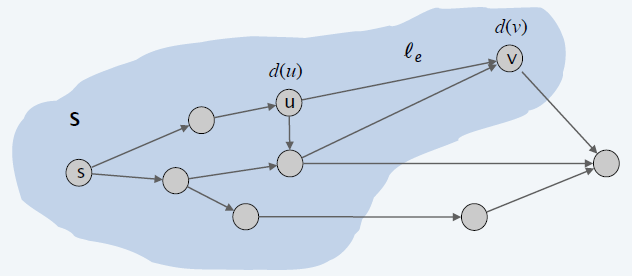
\includegraphics[scale=0.7]{figures/Dijkstra.png}
	\caption{Dijkstra算法示意图}
	\label{fig:Dijkstra}
\end{figure}
如图\ref{fig:Dijkstra},该图中s是起点,最右侧的点是终点。$d(u)$表示从点$s$到点$u$的最短距离。之后执行如下操作:\\
(1)初始化$S={s},d(s)=0$;\\
(2)反复寻找未探索过的点v,使得$\min\quad\pi(v)$,将$v$添加到$S$中,并且$d(v)=\pi(v)$,其中
$$\pi(v)=\min_{e=(u,v):u\in S}d(u)+distance(arg\min_{e=(u,v):u\in S}d(u),v)$$
最终当终点属于$S$时,可以知道起点到终点的最短路径长度,从而问题求解。\\\\
可以看出,问题一的核心关键在于玩家是否前往矿山挖矿、在矿山连续挖几天矿、在挖矿之后是否需要前往村庄补给物资以及是否可以在矿山和村庄之间往返。我们将问题作如下简化:

选取图中起点、终点、村庄和矿山作为特殊点,利用Dijkstra算法计算出每两个特殊点之间的最短路径(即不考虑沙暴天气的影响下,所需最少的天数),如图\ref{fig:map1}:
\begin{figure}[H]
	\centering
	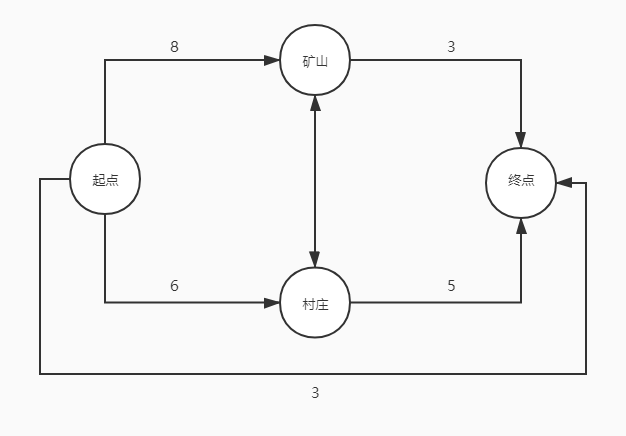
\includegraphics[scale=0.5]{figures/map1new.jpg}
	\caption{简化后的Map1}
	\label{fig:map1}
\end{figure}
该图是一个完全图(即图中每两点之间都有一条边),且每条边上的数字代表着两个特殊点之间的最短路径(受天气影响可能会有变化)。其中:$P_0$代表起点,$P_1$代表村庄,$P_2$代表矿山,$P_3$代表终点。对于问题一,因为天气是预先给定的,整局游戏没有随机因素,所以我们假定玩家在游戏途中始终向着某个特殊点(终点、村庄、矿山)前进并且选择最合适的路径,而非漫无目的地随机移动,即游戏旅程由几条有向线段叠加而成:
\begin{equation}
	\overrightarrow{P}=\sum_{k=1}^{n}\overrightarrow{P_{i_k}P_{i_{k+1}}}
\end{equation}
其中$i_k\leqslant3,\quad k=1,2,\dots,n$.

%参考文献
\begin{thebibliography}{9}%宽度9

    

\end{thebibliography}

\end{document} 